\documentclass[10pt]{article}
\usepackage[margin=1in]{geometry}
\usepackage{graphicx}
\usepackage{booktabs}
\usepackage{caption}
\usepackage{subcaption}
\usepackage{float}
\usepackage{hyperref}
\usepackage{amsmath}
\usepackage{array}

\setlength{\parindent}{0pt}
\setlength{\parskip}{4pt}
\captionsetup{font=small, labelfont=bf}

\title{\vspace{-1.0cm}Interpretable Diabetes Risk Analysis in the Health and Retirement Study}
\author{Group 8}
\date{}

\begin{document}
\maketitle
\vspace{-0.8cm}

\section*{Introduction}

Diabetes is a major public health concern among older adults and is closely linked to cardiovascular disease, disability, health care spending, and quality of life. Many diabetes risk factors, including body mass index (BMI), smoking, and physical activity, are behavioral or metabolic features that may vary across demographic and socioeconomic groups. Standard regression models are useful for estimating average associations, but they can obscure nonlinear risk patterns and heterogeneous effects. For example, BMI may not have a constant linear association with diabetes risk across the full range of body size, and the association between physical activity and diabetes may differ by age, BMI, income, or race/ethnicity.

The objective of this project was to analyze diabetes risk patterns in a large cohort of older U.S. adults using both traditional statistical learning methods and interpretable machine learning. Rather than focusing only on maximizing a prediction score, we aimed to understand which factors were most associated with diabetes, whether age and BMI had nonlinear relationships with risk, and whether the association between physical activity and diabetes persisted after adjustment for measured confounders. We used logistic regression, penalized regression, tree-based models, a neural network, explainable boosting machines (EBMs), restricted cubic spline models, subgroup analyses, and inverse probability weighting (IPW) sensitivity analyses.

\section*{Methods}

\subsection*{Data source and study sample}

We used an analytic file derived from Wave 10 of the Health and Retirement Study (HRS), a nationally representative longitudinal survey of U.S. adults over age 50. The source file was a Stata data set containing a previously constructed HRS analytic sample with diabetes status, physical activity, demographic covariates, socioeconomic covariates, BMI, smoking, urban residence, a propensity score for physical activity, and an inverse probability weight. We converted the Stata file to a project-level CSV file and retained one row per respondent. The final analytic data set contained 20,114 respondents and 14 columns, including an individual identifier, the diabetes outcome, 10 analysis predictors, the propensity score, and the IPW weight.

The binary outcome was self-reported diabetes status, defined as whether the respondent reported that a doctor had ever told them they had diabetes or high blood sugar. The main exposure of scientific interest was vigorous physical activity, coded as any vigorous activity versus none. Other predictors were sex, age, race/ethnicity, education, marital status, BMI, household income, smoking status, and urban residence. Race/ethnicity was coded as non-Hispanic White, non-Hispanic Black, Hispanic, or other. Education, marital status, and income were treated as categorical variables. Age and BMI were treated as continuous variables in regression and machine learning models. The propensity score and IPW variables were retained only for sensitivity analyses of the physical activity association and were excluded from ordinary prediction models.

\subsection*{Pre-processing}

All binary and categorical variables were converted to integer-coded categories before modeling. The final analytic file had no missing values, but the modeling pipeline still used explicit imputation steps so that the scripts would remain stable if the data were updated. For scikit-learn and PyTorch models, continuous variables were median-imputed and standardized, while categorical variables were most-frequent-imputed and one-hot encoded with unseen categories ignored at prediction time. This produced 26 post-encoding features for the neural network and other design-matrix-based models. For EBM models, we passed the original feature columns directly and specified feature types as nominal for categorical predictors and continuous for age and BMI. For statsmodels logistic regression analyses, categorical variables were represented using indicator variables, with the lowest coded level used as the reference category.

\begin{table}[H]
\centering
\caption{Summary statistics for the HRS analytic sample.}
\scriptsize
\begin{tabular}{lcc}
\toprule
Characteristic & N (\%) or mean (SD) & Median [IQR] \\
\midrule
Age, years & 66.9 (11.2) & 66.0 [57.0, 75.0] \\
BMI, kg/m$^2$ & 29.0 (6.4) & 28.1 [24.7, 32.2] \\
Diabetes &  &  \\
\quad No diabetes & 15,667 (77.9\%) &  \\
\quad Diabetes & 4,447 (22.1\%) &  \\
Physical activity &  &  \\
\quad No vigorous activity & 11,479 (57.1\%) &  \\
\quad Any vigorous activity & 8,635 (42.9\%) &  \\
Sex &  &  \\
\quad Male & 8,677 (43.1\%) &  \\
\quad Female & 11,437 (56.9\%) &  \\
Race/ethnicity &  &  \\
\quad Non-Hispanic White & 13,223 (65.7\%) &  \\
\quad Non-Hispanic Black & 3,786 (18.8\%) &  \\
\quad Hispanic & 2,491 (12.4\%) &  \\
\quad Other & 614 (3.1\%) &  \\
Education &  &  \\
\quad Less than high school & 3,944 (19.6\%) &  \\
\quad High school graduate & 6,829 (34.0\%) &  \\
\quad Some college & 4,926 (24.5\%) &  \\
\quad College and above & 4,415 (21.9\%) &  \\
Marital status &  &  \\
\quad Married & 11,667 (58.0\%) &  \\
\quad Separated/divorced & 3,523 (17.5\%) &  \\
\quad Widowed & 3,865 (19.2\%) &  \\
\quad Never married & 1,059 (5.3\%) &  \\
Household income &  &  \\
\quad <25k & 6,831 (34.0\%) &  \\
\quad 25k-49k & 5,377 (26.7\%) &  \\
\quad 50k-99k & 4,637 (23.1\%) &  \\
\quad 100k+ & 3,269 (16.3\%) &  \\
Ever smoker &  &  \\
\quad No & 8,691 (43.2\%) &  \\
\quad Yes & 11,423 (56.8\%) &  \\
Urban residence &  &  \\
\quad Suburban/rural & 9,781 (48.6\%) &  \\
\quad Urban & 10,333 (51.4\%) &  \\
\bottomrule
\end{tabular}
\end{table}

\subsection*{Prediction models}

We treated diabetes status as a binary classification outcome. For ordinary prediction models, we used a stratified 70\% training and 30\% test split with random seed 263, yielding 14,079 training observations and 6,035 test observations. The same split was used for logistic regression, elastic net logistic regression, random forest, gradient boosting, EBM, and PyTorch MLP models. The restricted cubic spline logistic model was used primarily as an inference model and was fit on the full analytic sample so that adjusted curves and odds ratios used all available observations.

Logistic regression was used as a baseline linear classifier. We fit an unpenalized logistic regression with class-balanced weights and a maximum of 5,000 iterations. We then fit an elastic net logistic regression using 5-fold cross-validation within the training set, optimizing ROC AUC over 10 inverse-penalty values and three mixing parameters ($\alpha=0.1,0.5,0.9$). The selected elastic net model used $C=0.046$ and $\alpha=0.9$, indicating a strong lasso component. Class-balanced weights were used in both logistic models because diabetes cases represented about 22\% of the sample.

Random forest was included to capture nonlinearities and interactions without imposing a parametric structure. The final model used 600 trees, square-root feature sampling at each split, a minimum leaf size of 10, class-balanced bootstrap subsampling, and random seed 263. We used these settings to keep individual trees from becoming too unstable while still allowing flexible splits across demographic, socioeconomic, and health variables. We also saved impurity-based feature importance values as a secondary description of which encoded predictors were most often used by the forest.

Gradient boosting was fit using a histogram-based gradient boosting classifier. The model used 250 boosting iterations, learning rate 0.04, L2 regularization 0.1, minimum leaf size 25, and random seed 263. Compared with the random forest, this model builds trees sequentially and can learn additive nonlinear structure through boosted corrections. We chose a modest learning rate and regularization to reduce overfitting because the number of predictors was relatively small but the outcome was imbalanced.

The EBM was fit using the \texttt{interpret} package's \texttt{ExplainableBoostingClassifier}. We used main effects only (\texttt{interactions=0}), learning rate 0.03, 256 maximum bins, and random seed 263. This model can be viewed as a generalized additive model learned by boosting, where each feature has its own estimated contribution function on the log-odds scale. We chose the no-interaction EBM as the main interpretable machine learning model because it provides transparent term-level plots while still allowing nonlinear shapes for continuous predictors.

The neural network was implemented in PyTorch as a multilayer perceptron with hidden layer sizes 128, 64, and 32. The first two hidden layers used batch normalization and ReLU activation, with dropout rates 0.25 and 0.15. The model was trained with weighted binary cross-entropy, AdamW optimization, learning rate 0.001, and weight decay 0.01. Within the 70\% training set, 20\% was held out as a validation set for early stopping. Training was allowed up to 400 epochs with patience 40; the final run stopped after 44 epochs and restored the weights with the best validation loss.

Model performance was evaluated using AUC, PR-AUC, accuracy, sensitivity, specificity, precision, F1 score, Brier score, and log loss. AUC summarizes ranking ability across classification thresholds, while PR-AUC is more sensitive to performance for the diabetes-positive class. Brier score and log loss were included because predicted probabilities are important for risk interpretation, not only classification. Accuracy, sensitivity, specificity, precision, and F1 score were calculated at a default probability threshold of 0.5. Because the project goal was analysis and insight rather than a competition leaderboard, these metrics were used to understand model behavior rather than to choose the single highest-scoring black-box model.

\subsection*{Interpretability and sensitivity analyses}

To estimate nonlinear adjusted risk patterns, we fit a binomial generalized linear model with restricted cubic spline terms for age and BMI. Each spline used four degrees of freedom. The model adjusted for physical activity, sex, race/ethnicity, education, marital status, income, smoking, and urban residence. We generated adjusted diabetes probability curves by varying age or BMI over the 1st to 99th percentile range while holding the other continuous variable at its median and categorical variables at their modal levels. We used likelihood ratio tests to compare the full spline model with reduced models that removed the age spline or BMI spline terms.

We used EBM explanations to complement the regression analyses. Global importance was defined by the mean absolute contribution of each term, and individual term plots were saved for every predictor. These plots show how each variable changes the predicted diabetes log-odds while preserving the additive structure of the model. In the main report, we used the global importance ranking and selected term plots for physical activity, age, and BMI, because these terms were most directly tied to the scientific question.

To study heterogeneity in the physical activity association, we fit adjusted logistic regression models within subgroups defined by sex, age group (51--64 versus 65+), BMI category (normal/underweight, overweight, obese), income group (low/mid versus higher income), and race/ethnicity. Each subgroup model used the same adjustment set as the primary logistic model when estimable. We also fit interaction models adding product terms between physical activity and sex, age, BMI, income, or race/ethnicity. The main subgroup estimand was the adjusted odds ratio for diabetes comparing physically active versus inactive respondents.

Finally, because physical activity was observational rather than randomized, we conducted IPW sensitivity analyses. We used the existing IPW variable in the analytic file, which had mean 2.00 and maximum 14.86. We compared four logistic regression estimates for physical activity: unweighted unadjusted, unweighted covariate-adjusted, IPW marginal, and IPW covariate-adjusted. Weighted logistic models used binomial GLMs with robust HC3 standard errors. We also fit unweighted and IPW-weighted EBMs on the full data to examine whether the learned physical activity contribution changed after weighting.

\section*{Results}

\subsection*{Model comparison}

The models showed moderate discrimination. Among held-out prediction models, EBM had the highest test AUC (0.702), followed by MLP (0.700), gradient boosting (0.699), random forest (0.697), and the logistic models (0.695). The restricted cubic spline logistic model had an apparent full-sample AUC of 0.711 and the best Brier score, but this value is best interpreted as an inference-model summary rather than a directly comparable held-out test result. Overall, the performance differences were small, suggesting that the main value of the analysis comes from interpretability and pattern discovery rather than a large gain in pure prediction accuracy.

\begin{table}[H]
\centering
\caption{Model performance. Prediction models are evaluated on the held-out test set; the spline logistic model is summarized on the full analytic sample because it was fit as an inference model.}
\scriptsize
\begin{tabular}{lrrrrrrr}
\toprule
Model & AUC & PR-AUC & Brier & Log loss & Accuracy & Sens. & Spec. \\
\midrule
Spline logistic & 0.711 & 0.396 & 0.156 & 0.479 & 0.780 & 0.094 & 0.975 \\
EBM & 0.702 & 0.394 & 0.157 & 0.482 & 0.784 & 0.076 & 0.984 \\
PyTorch MLP & 0.700 & 0.385 & 0.220 & 0.627 & 0.610 & 0.690 & 0.588 \\
Gradient boosting & 0.699 & 0.386 & 0.157 & 0.484 & 0.781 & 0.050 & 0.989 \\
Random forest & 0.697 & 0.384 & 0.199 & 0.580 & 0.680 & 0.579 & 0.709 \\
Elastic net logistic & 0.695 & 0.379 & 0.220 & 0.632 & 0.642 & 0.623 & 0.648 \\
Logistic regression & 0.695 & 0.379 & 0.220 & 0.633 & 0.640 & 0.623 & 0.645 \\
\bottomrule
\end{tabular}
\end{table}

\begin{figure}[H]
\centering
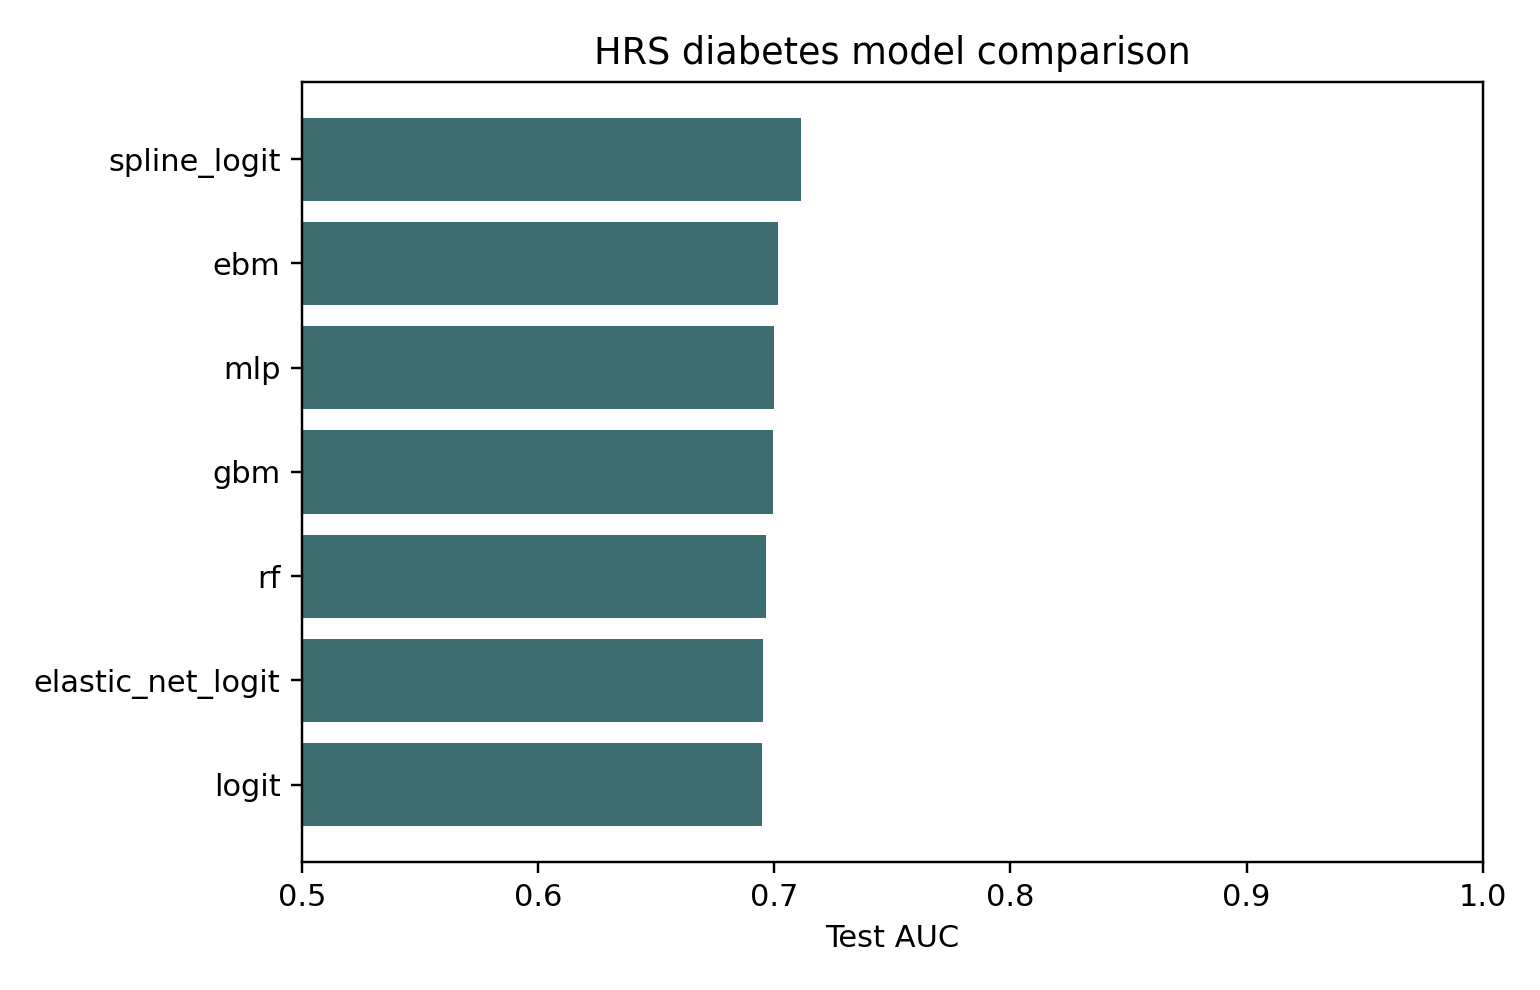
\includegraphics[width=0.72\linewidth]{figures/auc.png}
\caption{Comparison of test-set AUC across prediction models.}
\end{figure}

We selected the restricted cubic spline model and EBM together as the most useful models for inference. The spline model provided a familiar epidemiologic regression framework, clear adjusted odds ratios, and formal tests of nonlinear age and BMI effects. The EBM provided the best held-out AUC among the machine learning models while preserving a transparent additive explanation of variable importance and variable-level risk patterns.

\subsection*{Key predictors and nonlinear risk patterns}

The EBM ranked BMI, age, physical activity, race/ethnicity, income, and sex as the most important terms. This ranking aligned with the spline logistic model, in which age and BMI had strong nonlinear associations with diabetes risk. Likelihood ratio tests strongly supported retaining nonlinear spline terms for both age and BMI (age: $\chi^2=246.7$, $p<0.001$; BMI: $\chi^2=901.0$, $p<0.001$). The BMI curve showed a clear increase in adjusted diabetes probability at higher BMI values. The age curve also showed a nonlinear relationship, consistent with the idea that diabetes risk in older adults is not fully captured by a simple linear age effect.

\begin{figure}[H]
\centering
\begin{subfigure}{0.48\linewidth}
\centering
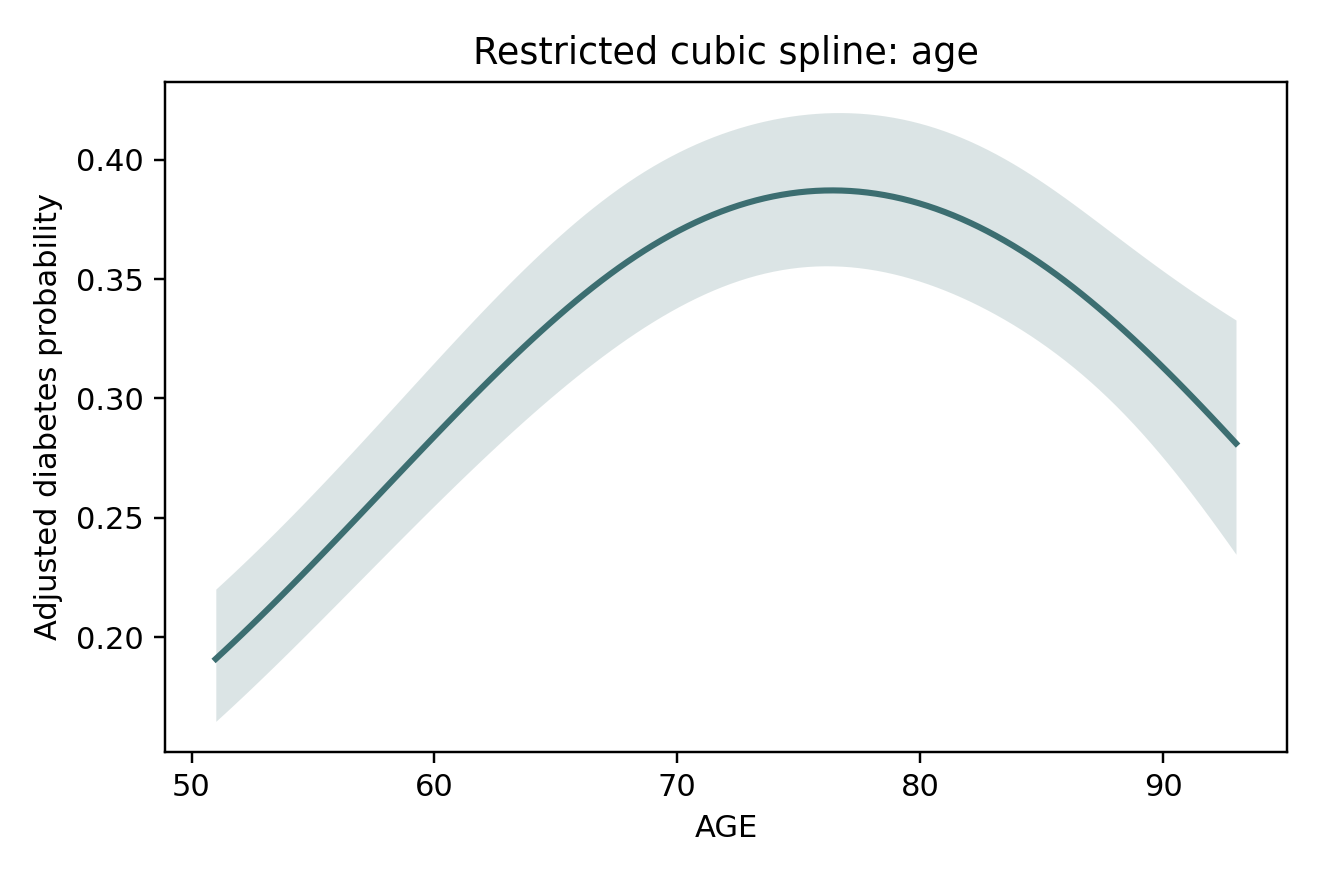
\includegraphics[width=\linewidth]{figures/age_curve.png}
\caption{Age}
\end{subfigure}
\begin{subfigure}{0.48\linewidth}
\centering
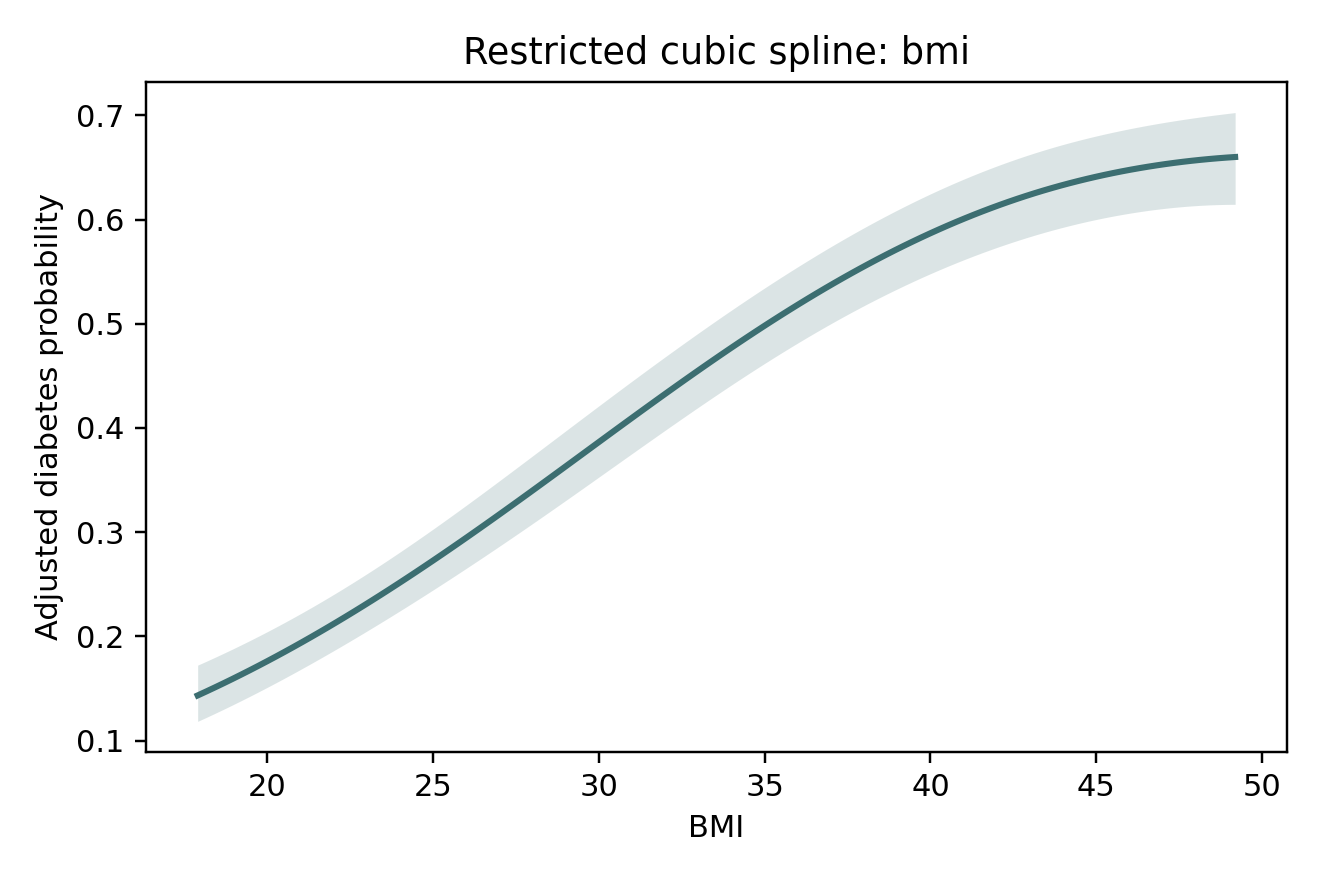
\includegraphics[width=\linewidth]{figures/bmi_curve.png}
\caption{BMI}
\end{subfigure}
\caption{Adjusted diabetes probability curves from restricted cubic spline logistic regression.}
\end{figure}

In the adjusted spline logistic model, any vigorous physical activity was associated with lower diabetes odds (OR=0.64, 95\% CI: 0.59--0.69). Higher education and higher income were also associated with lower diabetes odds, while non-Hispanic Black, Hispanic, and other race/ethnicity categories had higher odds compared with non-Hispanic White respondents after adjustment.

\begin{table}[H]
\centering
\caption{Selected adjusted odds ratios from the spline logistic model.}
\scriptsize
\begin{tabular}{lrr}
\toprule
Variable & Adjusted OR & 95\% CI \\
\midrule
Any vigorous activity & 0.64 & [0.59, 0.69] \\
Female & 0.73 & [0.67, 0.78] \\
Non-Hispanic Black & 1.66 & [1.51, 1.83] \\
Hispanic & 1.74 & [1.55, 1.95] \\
Other race/ethnicity & 1.91 & [1.56, 2.34] \\
College and above & 0.78 & [0.69, 0.88] \\
Household income $\ge$100k & 0.60 & [0.52, 0.70] \\
Ever smoker & 0.99 & [0.92, 1.07] \\
Urban residence & 0.92 & [0.85, 0.99] \\
\bottomrule
\end{tabular}
\end{table}

\subsection*{Subgroup and interaction analyses}

The inverse association between physical activity and diabetes was present in most subgroups. The overall adjusted OR was 0.66. The association appeared strongest among respondents with normal or underweight BMI (OR=0.53), intermediate among overweight respondents (OR=0.63), and weaker among obese respondents (OR=0.73). The physical activity by BMI interaction was statistically significant ($p<0.001$), suggesting that the association between activity and diabetes risk differs across BMI. Race/ethnicity interactions were also observed, though the smallest race/ethnicity subgroup had wide uncertainty.

\begin{figure}[H]
\centering
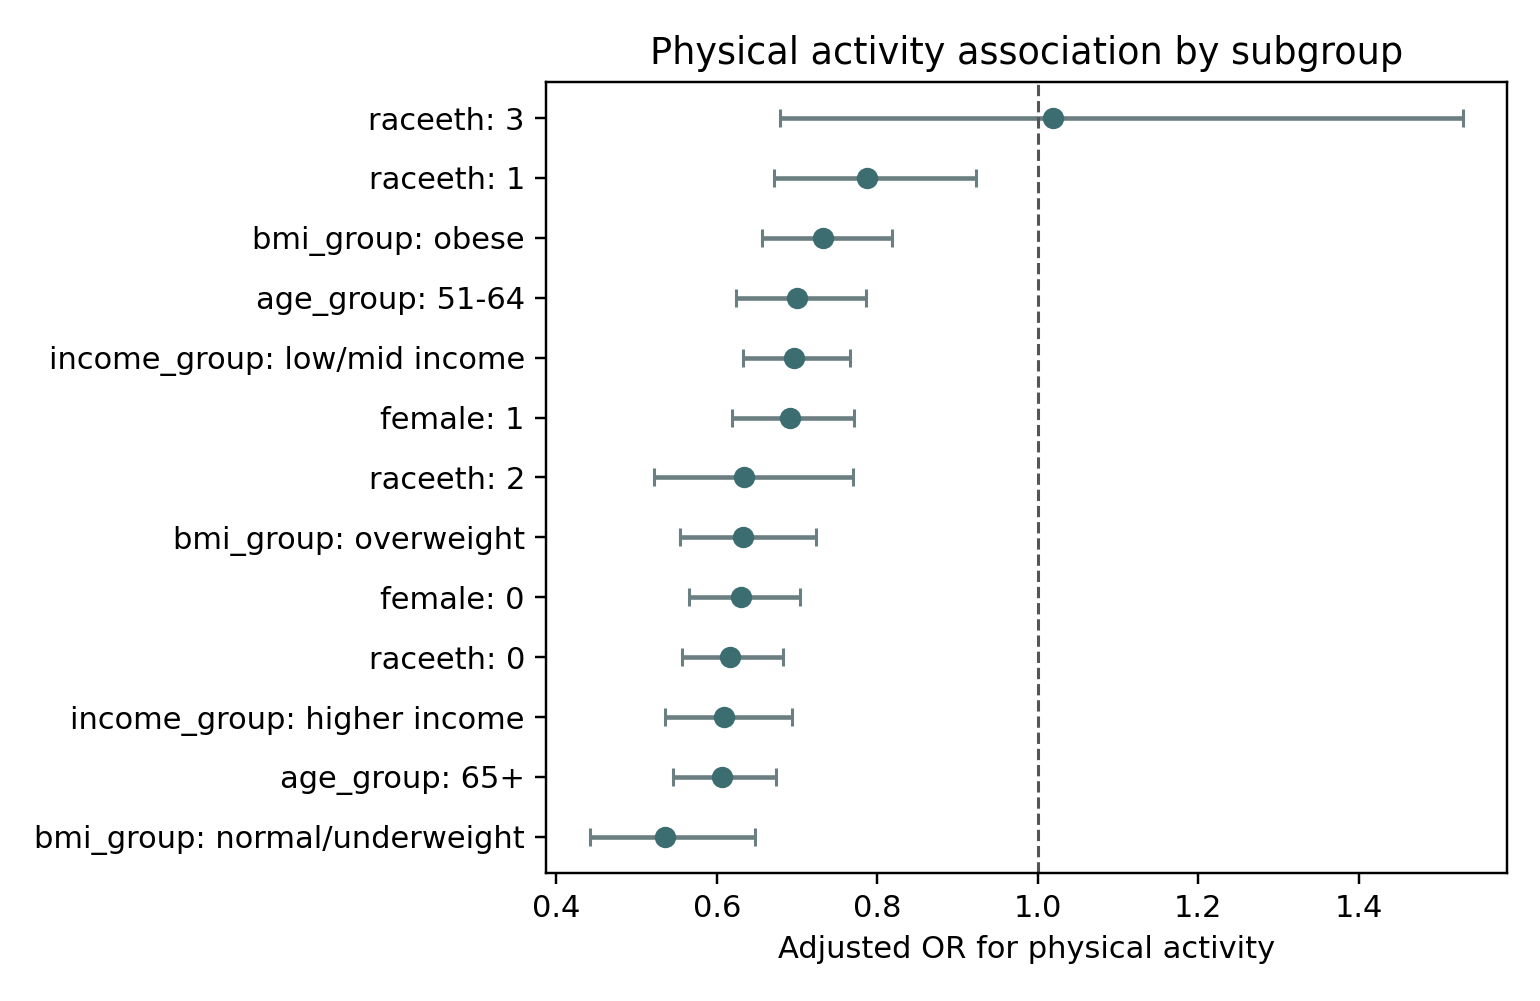
\includegraphics[width=0.78\linewidth]{figures/subgroup_or.png}
\caption{Adjusted odds ratios for physical activity by subgroup. Values below 1 indicate lower odds of diabetes among physically active respondents.}
\end{figure}

\subsection*{IPW sensitivity analysis}

The unadjusted association between physical activity and diabetes was stronger than the adjusted association (unweighted unadjusted OR=0.54 versus unweighted adjusted OR=0.66), indicating confounding by demographic, socioeconomic, and health-related covariates. However, the association persisted after IPW adjustment. The IPW marginal OR was 0.69 and the IPW adjusted OR was 0.67. The EBM physical activity contribution also remained protective after weighting, although the weighted EBM showed a more symmetric contribution pattern.

\begin{table}[H]
\centering
\caption{Physical activity odds ratios from unweighted and IPW-weighted analyses.}
\scriptsize
\begin{tabular}{lrr}
\toprule
Analysis & OR & 95\% CI \\
\midrule
Unweighted, unadjusted & 0.54 & [0.50, 0.58] \\
Unweighted, adjusted & 0.66 & [0.61, 0.71] \\
IPW, marginal & 0.69 & [0.66, 0.73] \\
IPW, adjusted & 0.67 & [0.64, 0.70] \\
\bottomrule
\end{tabular}
\end{table}

\begin{figure}[H]
\centering
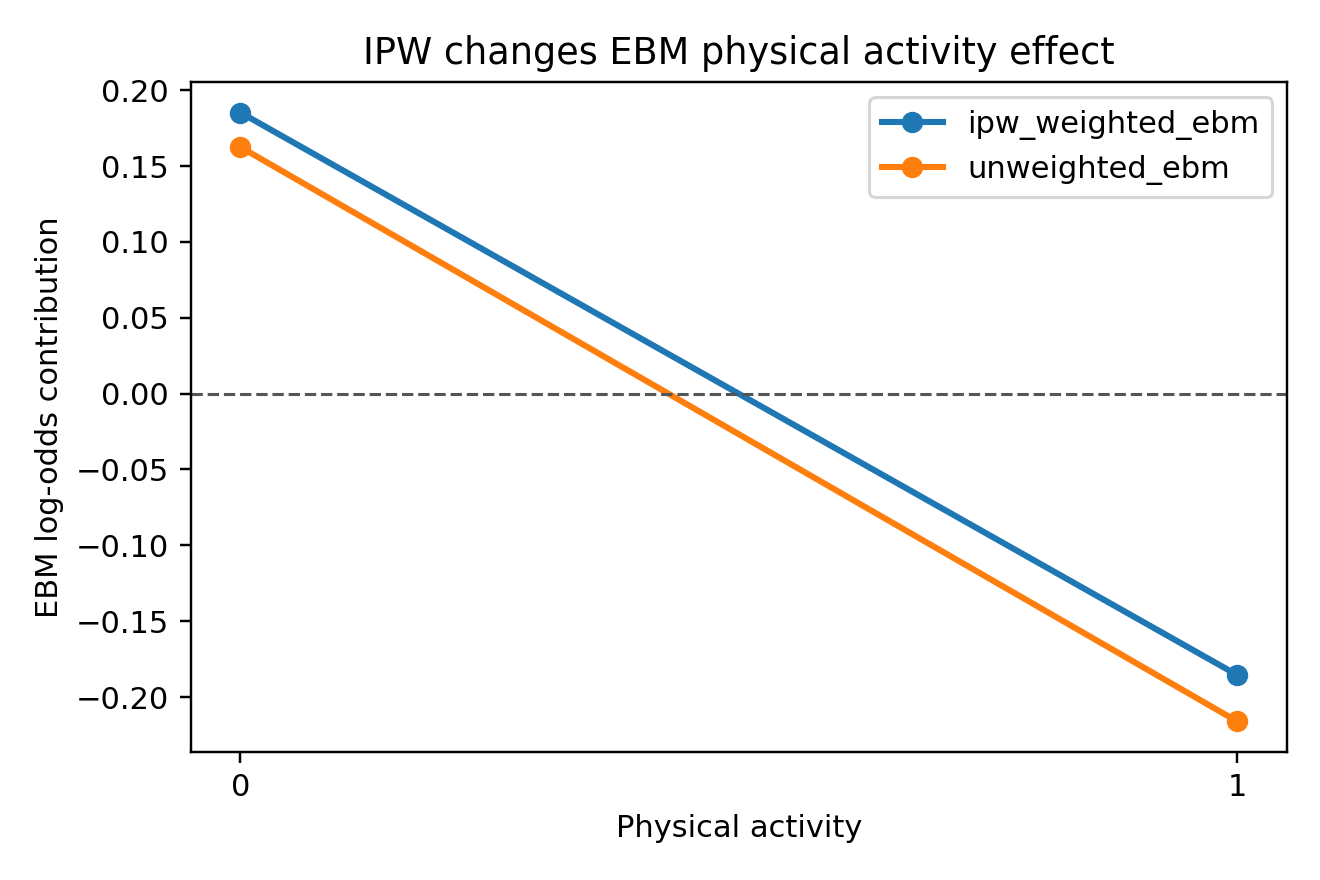
\includegraphics[width=0.65\linewidth]{figures/ipw_ebm_physical_activity.png}
\caption{EBM log-odds contribution for physical activity before and after IPW weighting.}
\end{figure}

\section*{Discussion}

This analysis used HRS data to examine diabetes risk patterns among older adults with a focus on interpretability. The main findings were that BMI and age had strong nonlinear associations with diabetes risk, physical activity was consistently associated with lower diabetes odds, and the physical activity association remained after covariate adjustment and IPW weighting. The spline logistic model and EBM were the most useful models for this project because they balanced performance with interpretability. The spline model offered adjusted odds ratios and smooth risk curves, while the EBM offered a transparent machine learning view of feature importance and covariate contributions.

The model comparison suggested that the available variables contain meaningful but limited predictive information. AUC values clustered around 0.69--0.71, which is reasonable for a model based only on demographic, socioeconomic, BMI, smoking, urbanicity, and physical activity variables. We would not interpret these models as clinical diagnostic tools. Instead, they are better viewed as tools for characterizing risk patterns and generating public-health insights.

The fairness implications of the analysis are important. HRS is designed to represent older U.S. adults, but diabetes risk and physical activity are shaped by structural factors including socioeconomic position, built environment, access to care, and historical inequities. Race/ethnicity and income were important predictors, but these variables should not be interpreted as biological causes. They likely capture broader social and environmental conditions. Model use should therefore focus on understanding population risk patterns and inequities, not assigning blame or making individual-level decisions without context.

Several limitations remain. Diabetes and physical activity were self-reported, so measurement error is possible. The analysis was cross-sectional and cannot establish temporality or causality. IPW adjusts only for measured confounders and may be sensitive to model specification and extreme weights. The physical activity variable was binary and did not capture detailed dose, duration, or type of activity. Finally, the prediction models used a limited set of variables; adding medication history, prior health conditions, diet, family history, biomarkers, or longitudinal HRS measures could improve both prediction and interpretation.

Overall, the project supports a clear substantive conclusion: among older adults in HRS, diabetes risk is strongly patterned by BMI and age in nonlinear ways, and vigorous physical activity is associated with lower diabetes odds even after adjustment for measured covariates. Interpretable statistical learning methods were especially valuable because they allowed us to move beyond overall prediction metrics and examine the shape and heterogeneity of these associations.

\section*{Group Contributions}

TODO

\section*{References}

\begin{enumerate}
\item Sonnega A, Faul JD, Ofstedal MB, Langa KM, Phillips JWR, Weir DR. Cohort profile: the Health and Retirement Study (HRS). \textit{International Journal of Epidemiology}. 2014;43(2):576--585.
\item American Diabetes Association. Diagnosis and classification of diabetes mellitus. \textit{Diabetes Care}. 2014;37(Supplement 1):S81--S90.
\item Hastie T, Tibshirani R. Generalized additive models. \textit{Statistical Science}. 1986;1(3):297--310.
\item Lou Y, Caruana R, Gehrke J, Hooker G. Accurate intelligible models with pairwise interactions. Proceedings of the 19th ACM SIGKDD International Conference on Knowledge Discovery and Data Mining. 2013.
\item Rosenbaum PR, Rubin DB. The central role of the propensity score in observational studies for causal effects. \textit{Biometrika}. 1983;70(1):41--55.
\end{enumerate}

\clearpage
\appendix
\section*{Appendix: Supplemental Model Figures}

The following figures provide additional method-specific diagnostics and visual summaries. They are included as supplemental material because they support the analyses but are not essential to the main narrative.

\begin{figure}[H]
\centering
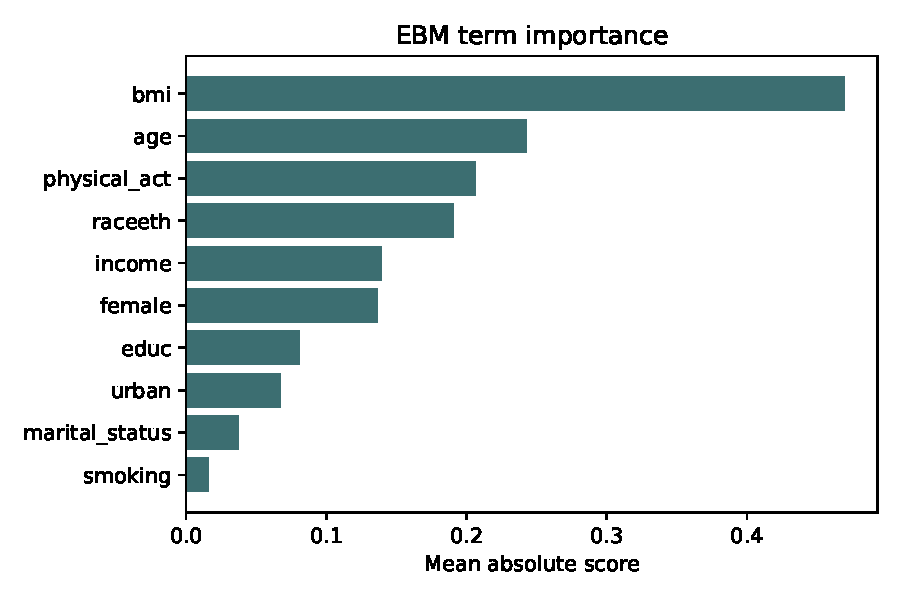
\includegraphics[width=0.70\linewidth]{figures/ebm_global.pdf}
\caption{Supplemental Figure A1. EBM global term importance.}
\end{figure}

\begin{figure}[H]
\centering
\begin{subfigure}{0.48\linewidth}
\centering
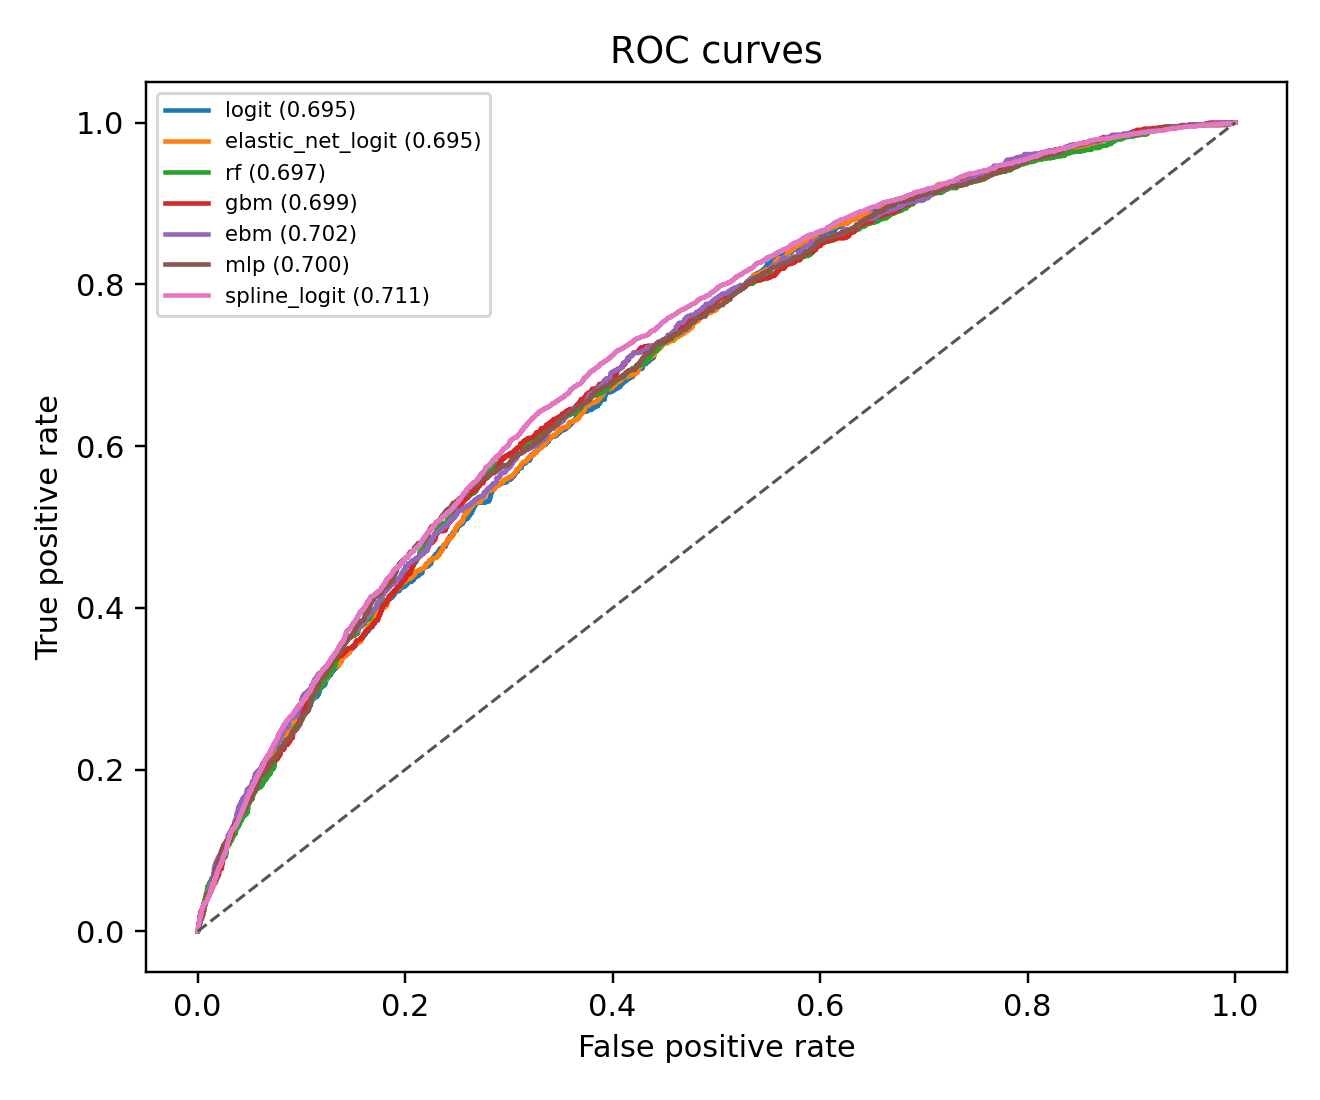
\includegraphics[width=\linewidth]{figures/roc.png}
\caption{ROC curves}
\end{subfigure}
\begin{subfigure}{0.48\linewidth}
\centering
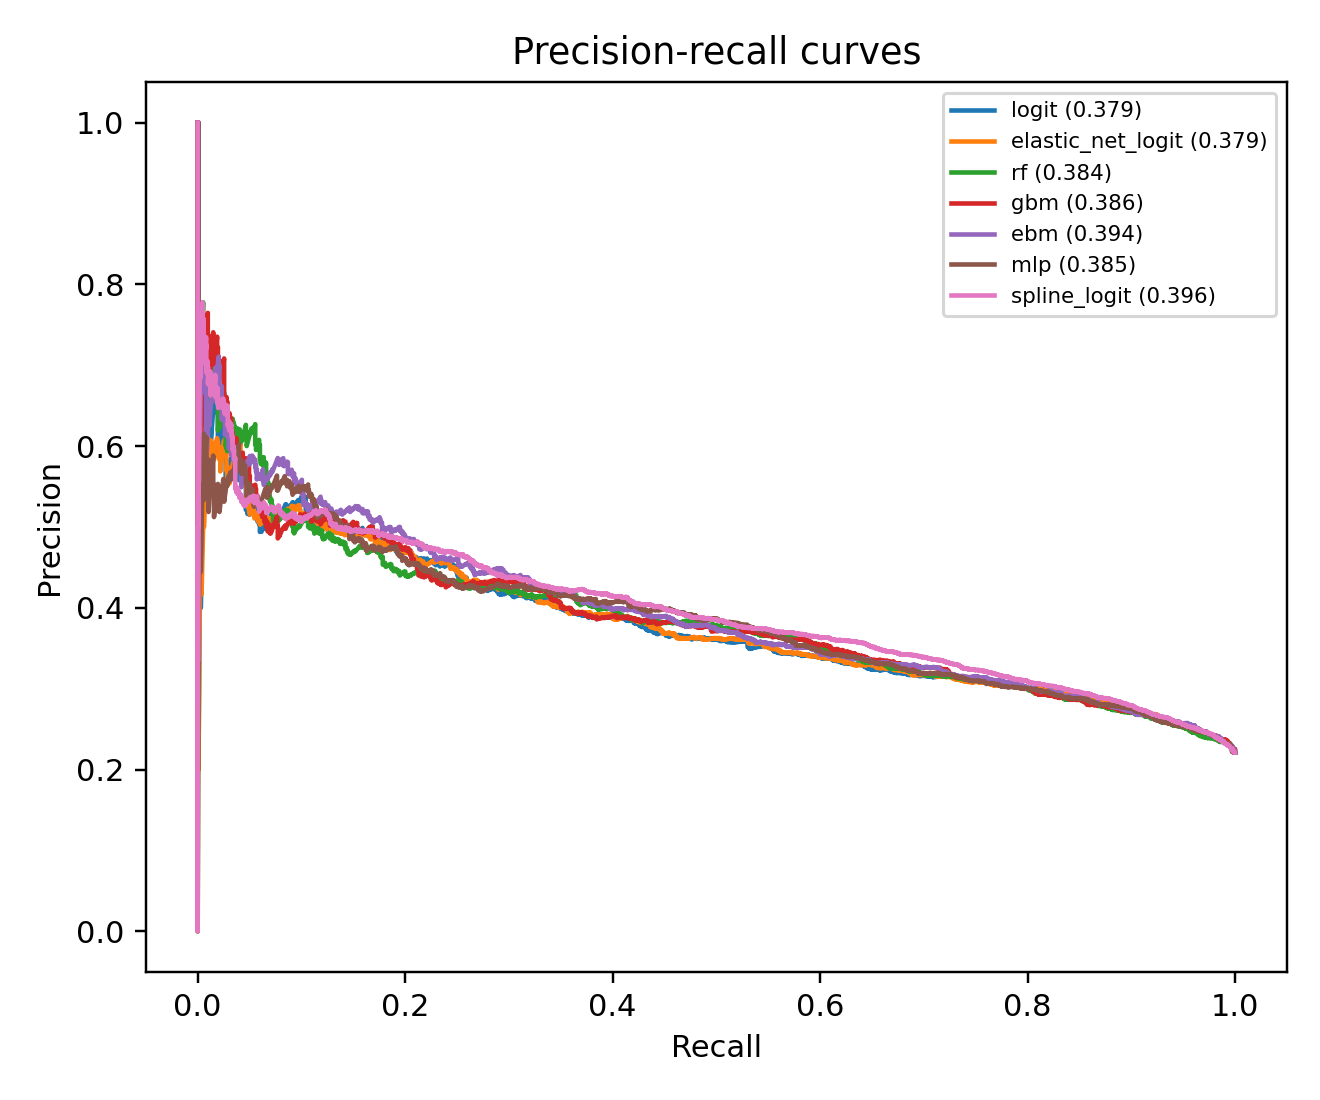
\includegraphics[width=\linewidth]{figures/pr.png}
\caption{Precision-recall curves}
\end{subfigure}
\caption{Supplemental Figure A2. Discrimination curves across prediction models.}
\end{figure}

\begin{figure}[H]
\centering
\begin{subfigure}{0.48\linewidth}
\centering
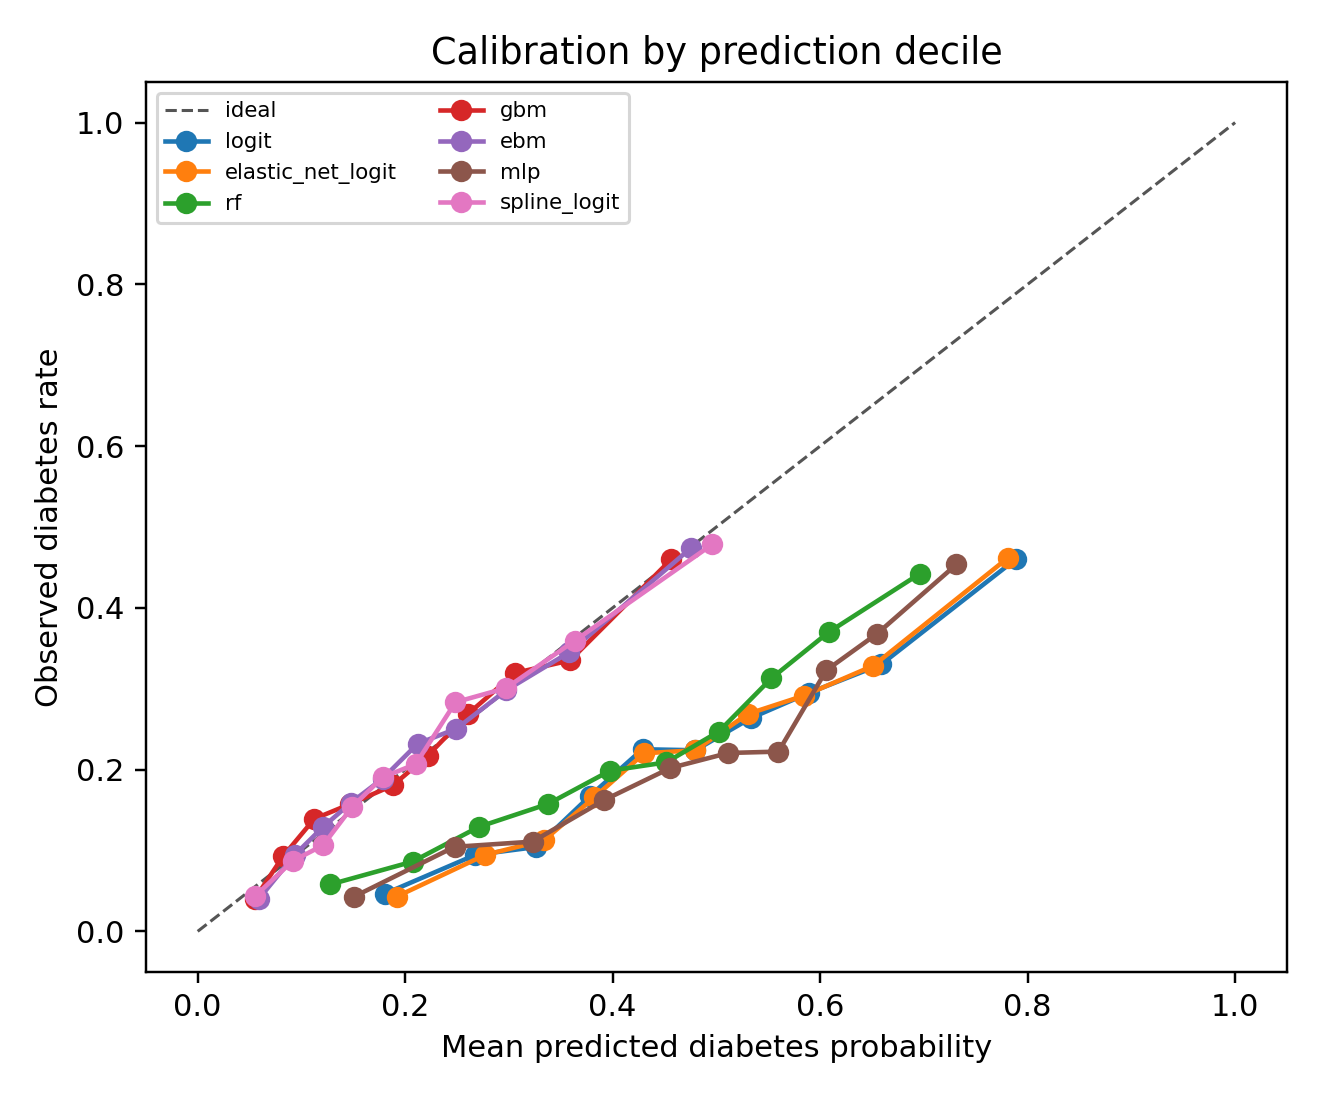
\includegraphics[width=\linewidth]{figures/calib.png}
\caption{Calibration by decile}
\end{subfigure}
\begin{subfigure}{0.48\linewidth}
\centering
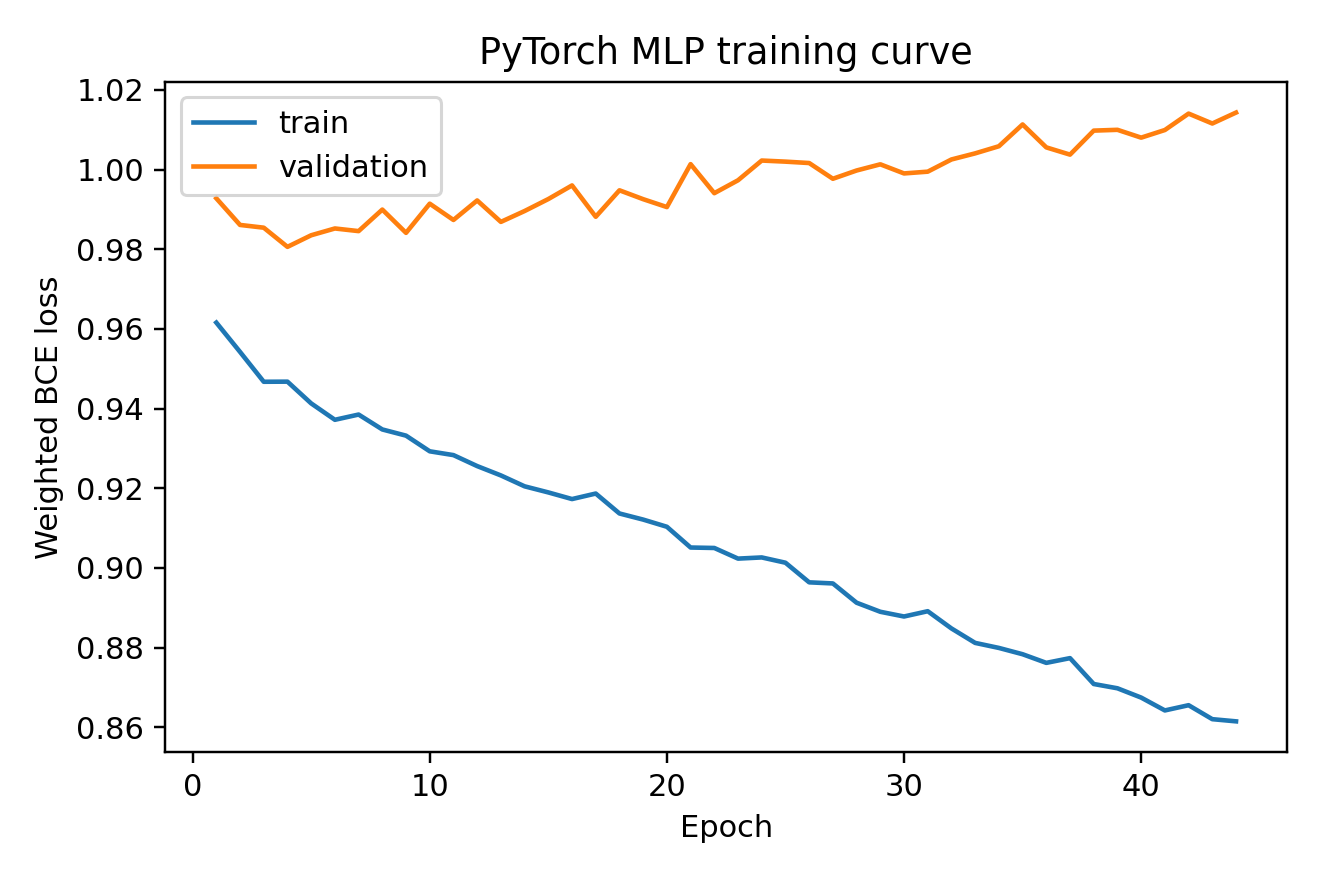
\includegraphics[width=\linewidth]{figures/nn_loss.png}
\caption{PyTorch MLP loss curve}
\end{subfigure}
\caption{Supplemental Figure A3. Calibration and neural network training diagnostics.}
\end{figure}

\begin{figure}[H]
\centering
\begin{subfigure}{0.32\linewidth}
\centering
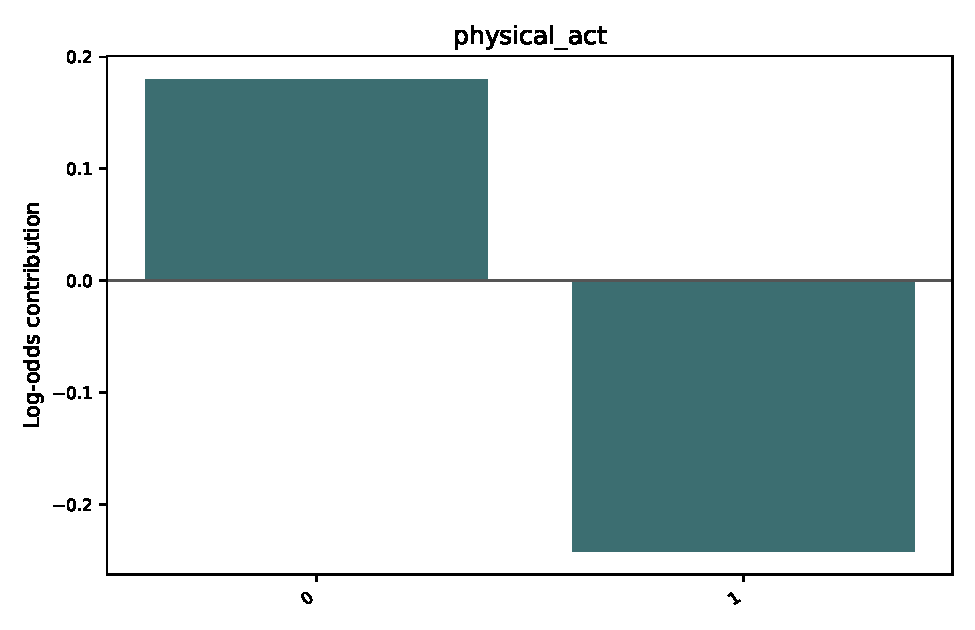
\includegraphics[width=\linewidth]{figures/ebm_physical_act.pdf}
\caption{Physical activity}
\end{subfigure}
\begin{subfigure}{0.32\linewidth}
\centering
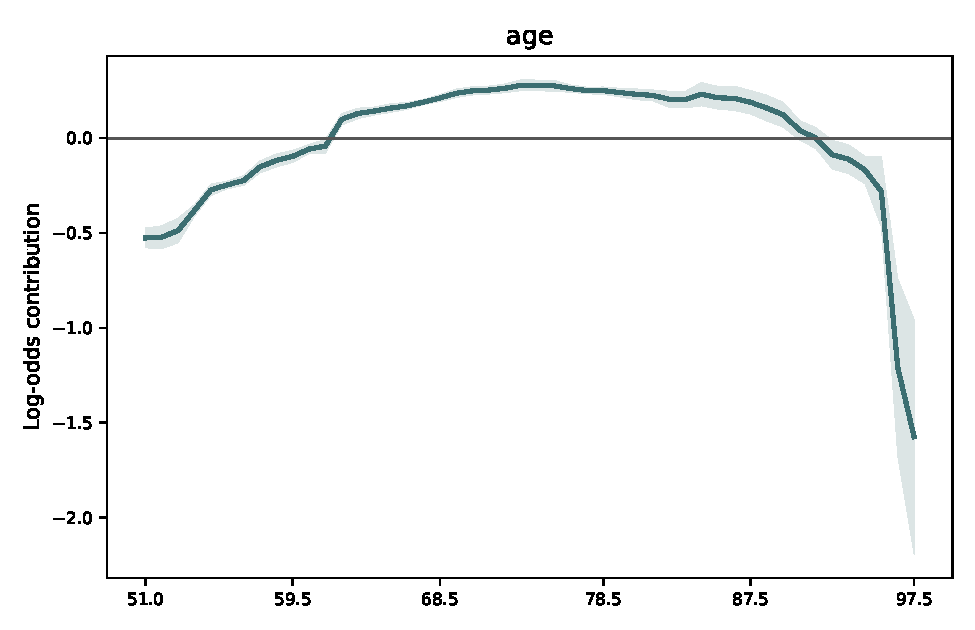
\includegraphics[width=\linewidth]{figures/ebm_age.pdf}
\caption{Age}
\end{subfigure}
\begin{subfigure}{0.32\linewidth}
\centering
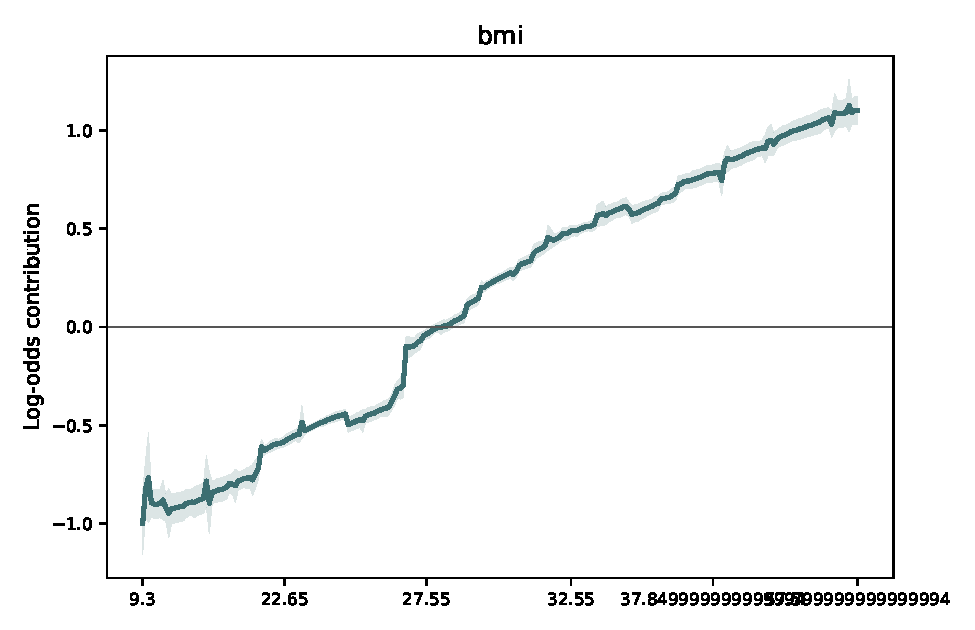
\includegraphics[width=\linewidth]{figures/ebm_bmi.pdf}
\caption{BMI}
\end{subfigure}
\caption{Supplemental Figure A4. Selected EBM term effects on the diabetes log-odds scale.}
\end{figure}

\end{document}
